\documentclass[a4paper,11pt]{article}

% ----------------- Packages -----------------
\usepackage[utf8]{inputenc}
\usepackage[T1]{fontenc}
\usepackage[english]{babel}
\usepackage{geometry}
\usepackage{amsmath}
\usepackage{graphicx}
\usepackage{tikz}
\usepackage{listings}
\usepackage{xcolor}
\usepackage{hyperref}

\geometry{margin=2.5cm}

% ----------------- Code style -----------------
\lstset{
    language=C++,
    basicstyle=\ttfamily\small,
    keywordstyle=\color{blue},
    commentstyle=\color{gray},
    stringstyle=\color{red!70!black},
    numbers=left,
    numberstyle=\tiny,
    stepnumber=1,
    frame=single,
    breaklines=true,
    showstringspaces=false,
    tabsize=4,
    captionpos=b
}

% ----------------- TikZ styles -----------------
\usetikzlibrary{positioning,arrows.meta,shapes.geometric}
\tikzset{
    stage/.style={
        rectangle, rounded corners,
        draw, minimum width=2.5cm,
        minimum height=1.0cm,
        align=center, font=\small, fill=blue!5
    },
    data/.style={
        trapezium, trapezium left angle=70,
        trapezium right angle=110,
        draw, minimum width=2.6cm,
        minimum height=1.0cm,
        align=center, font=\small, fill=green!5
    }
}

% ----------------- Title -----------------
\title{\textbf{Multithreaded Word Count Using Mapper--Reducer Style}}
\author{Hoang Minh Quan\\ \small Student ID: 23BI14371}
\date{\today}

\begin{document}
\maketitle

\begin{abstract}
This report presents a small C++ application that counts word
frequencies in a text file using a mapper--reducer style design.
The program reads an input file, splits the text into chunks that are
processed in parallel by mapper threads, and then combines the
intermediate results with reducer threads before writing the
global word counts to an output file.
\end{abstract}

\tableofcontents
\newpage

% ----------------- Introduction -----------------
\section{Introduction}

Counting how often each word appears in a text is a simple but
representative problem for data-processing frameworks.
In this assignment, we implement a standalone C++ program that performs
word counting in parallel on a single machine.
The program is inspired by the MapReduce model: we use several
\emph{mapper} threads to create local word-count maps and several
\emph{reducer} threads to merge these partial results into a final map.

The implementation uses the C++ standard library, threads, and
\texttt{std::unordered\_map} to store word frequencies.  Input and
output are handled via standard text files.

% ----------------- Problem description -----------------
\section{Problem Description}

The goal is to build a command-line tool with the following behaviour:
\begin{itemize}
    \item read a text file given by the user;
    \item normalise words (convert to lowercase and remove non-alphabetic
          characters);
    \item count how many times each distinct word occurs;
    \item allow the user to configure how many mapper and reducer threads
          are used;
    \item store the word counts in a separate output file.
\end{itemize}

The provided example input file contains the sentence
\begin{quote}
\texttt{why do programmers prefer dark mode because light attracts bugs}
\end{quote}
and the expected output lists each word once together with its
frequency, for example:
\begin{quote}
\begin{verbatim}
attracts 1
because 1
bugs 1
dark 1
do 1
light 1
mode 1
prefer 1
programmers 1
why 1
\end{verbatim}
\end{quote}

% ----------------- System overview -----------------
\section{System Overview}

\subsection{High-level Design}

The program follows four main stages:
\begin{enumerate}
    \item \textbf{Load file:} the entire input file is read into a single
          string.
    \item \textbf{Map phase:} the text is partitioned into chunks, each
          processed by a mapper thread producing a local
          \texttt{(word, count)} map.
    \item \textbf{Shuffle phase:} intermediate pairs are grouped so that
          all counts of the same word are sent to the same reducer.
    \item \textbf{Reduce phase:} reducer threads accumulate final word
          counts and the result is written to the output file.
\end{enumerate}

\subsection{Illustration}

Figure~\ref{fig:architecture} illustrates the architecture of the
application.  A single input text is transformed into several mapper
chunks, aggregated via reducer threads, and finally written as a sorted
list of words and frequencies.

\begin{figure}[h!]
    \centering
    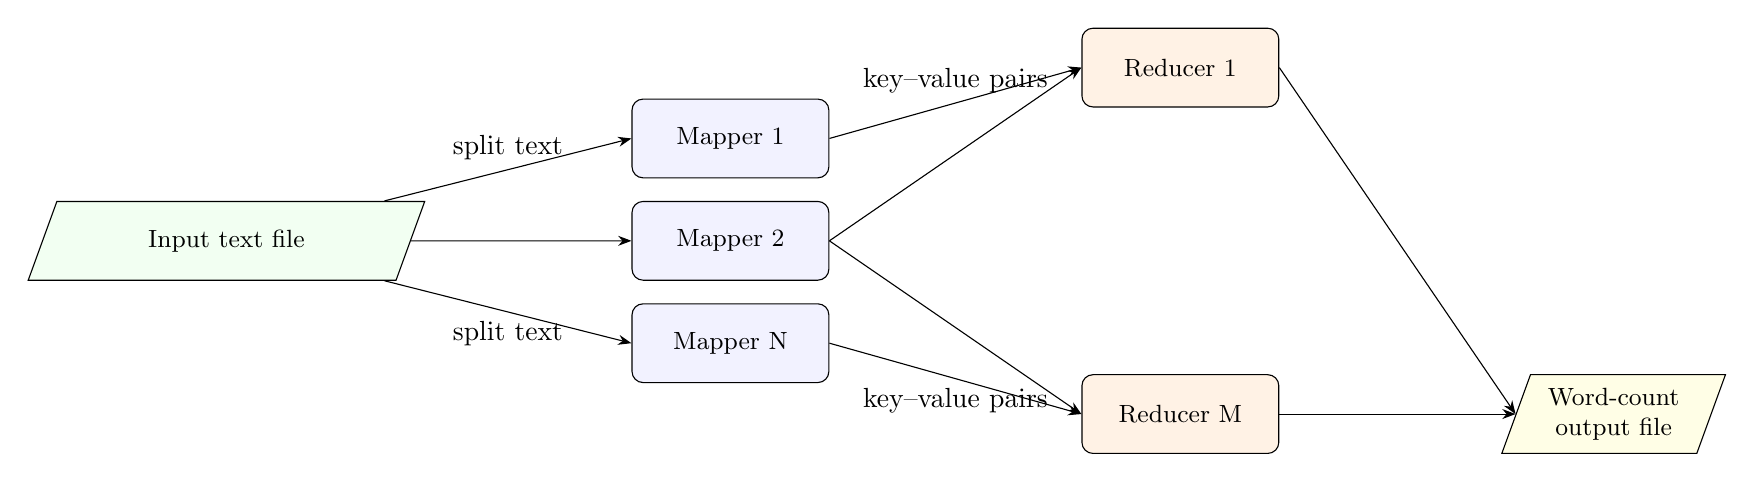
\begin{tikzpicture}[>=Stealth, node distance=1.5cm and 1.5cm]

        % Input
        \node[data] (input) {Input text file};

        % Mappers
        \node[stage, right=2.8cm of input, yshift=1.3cm] (m1) {Mapper 1};
        \node[stage, right=2.8cm of input] (m2) {Mapper 2};
        \node[stage, right=2.8cm of input, yshift=-1.3cm] (m3) {Mapper N};

        % Reducers
        \node[stage, right=3.2cm of m1, yshift=0.9cm, fill=orange!10] (r1) {Reducer 1};
        \node[stage, right=3.2cm of m3, yshift=-0.9cm, fill=orange!10] (r2) {Reducer M};

        % Output
        \node[data, right=3.0cm of r2, fill=yellow!10] (output) {Word-count\\output file};

        % Arrows
        \draw[->] (input) -- node[above]{split text} (m1.west);
        \draw[->] (input) -- (m2.west);
        \draw[->] (input) -- node[below]{split text} (m3.west);

        \draw[->] (m1.east) -- node[above]{key--value pairs} (r1.west);
        \draw[->] (m2.east) -- (r1.west);
        \draw[->] (m2.east) -- (r2.west);
        \draw[->] (m3.east) -- node[below]{key--value pairs} (r2.west);

        \draw[->] (r1.east) -- (output.west);
        \draw[->] (r2.east) -- (output.west);

    \end{tikzpicture}
    \caption{Mapper--reducer style architecture for the word-count tool.}
    \label{fig:architecture}
\end{figure}

% ----------------- Implementation -----------------
\section{Implementation Details}

\subsection{Word Normalisation and Splitting}

The function \texttt{normalize} converts characters to lowercase and
removes anything that is not an alphabetic letter.  A second helper
function, \texttt{split\_words}, walks through the input text, extracts
sequences of non-whitespace characters, normalises them, and returns a
vector of clean words.

\subsection{Mapper Threads}

Each mapper thread receives a substring (``chunk'') of the original text,
calls \texttt{split\_words} on that chunk, then builds a local
\texttt{unordered\_map<std::string,int>} that counts occurrences of each
word in the chunk.

To avoid cutting words in half, the code adjusts the chunk boundary to
the next whitespace character before launching the mapper.

\subsection{Reducer Threads}

After all mapper threads have finished, the program distributes the
intermediate \texttt{(word, count)} pairs to reducers.  A simple hash
partitioning scheme is used:
\begin{equation}
  \text{reducer\_id} = \text{hash}(\text{word}) \bmod \text{num\_reducers}.
\end{equation}
Each reducer accumulates the counts it receives into its own
\texttt{unordered\_map}.  Finally, these per-reducer maps are merged into
a single global map.

\subsection{Source Code Listing}

Listing~\ref{lst:wordcount} shows the full implementation of the program.

\begin{lstlisting}[caption={C++ implementation of the multithreaded word-count tool},
                   label={lst:wordcount}]
#include <algorithm>
#include <cctype>
#include <fstream>
#include <iostream>
#include <mutex>
#include <string>
#include <thread>
#include <unordered_map>
#include <utility>
#include <vector>

using MapperOutput = std::unordered_map<std::string, int>;
using ReducerOutput = std::unordered_map<std::string, int>;

std::mutex io_mutex;

std::string normalize(const std::string &w) {
    std::string res;
    for (char c : w) {
        if (std::isalpha(static_cast<unsigned char>(c))) {
            res.push_back(static_cast<char>(std::tolower(c)));
        }
    }
    return res;
}

std::vector<std::string> split_words(const std::string &text) {
    std::vector<std::string> words;
    std::string current;
    for (char c : text) {
        if (std::isspace(static_cast<unsigned char>(c))) {
            if (!current.empty()) {
                std::string norm = normalize(current);
                if (!norm.empty()) words.push_back(norm);
                current.clear();
            }
        } else {
            current.push_back(c);
        }
    }
    if (!current.empty()) {
        std::string norm = normalize(current);
        if (!norm.empty()) words.push_back(norm);
    }
    return words;
}

void mapper_worker(const std::string &chunk, MapperOutput &out_map) {
    auto words = split_words(chunk);
    for (const auto &w : words) {
        ++out_map[w];
    }
}

void reducer_worker(const std::vector<std::pair<std::string, int>> &pairs,
                    ReducerOutput &out_map) {
    for (const auto &p : pairs) {
        out_map[p.first] += p.second;
    }
}

int main(int argc, char **argv) {
    if (argc < 3) {
        std::cerr << "Usage: " << argv[0]
                  << " <input_file> <output_file> [num_mappers] [num_reducers]\n";
        return 1;
    }

    std::string input_file = argv[1];
    std::string output_file = argv[2];
    int num_mappers = (argc >= 4) ? std::stoi(argv[3]) : 4;
    int num_reducers = (argc >= 5) ? std::stoi(argv[4]) : 2;

    if (num_mappers <= 0 || num_reducers <= 0) {
        std::cerr << "Number of mappers and reducers must be > 0\n";
        return 1;
    }

    std::ifstream in(input_file, std::ios::binary);
    if (!in.is_open()) {
        std::cerr << "Cannot open input file: " << input_file << "\n";
        return 1;
    }
    std::string text((std::istreambuf_iterator<char>(in)),
                     std::istreambuf_iterator<char>());
    in.close();

    if (text.empty()) {
        std::cerr << "Input file is empty.\n";
        return 1;
    }

    std::vector<std::thread> mapper_threads;
    std::vector<MapperOutput> mapper_outputs(num_mappers);

    size_t chunk_size = text.size() / num_mappers;
    size_t start = 0;

    for (int i = 0; i < num_mappers; ++i) {
        size_t end = (i == num_mappers - 1) ? text.size() : start + chunk_size;

        if (end < text.size()) {
            while (end < text.size() &&
                   !std::isspace(static_cast<unsigned char>(text[end]))) {
                ++end;
            }
        }

        std::string chunk = text.substr(start, end - start);
        mapper_threads.emplace_back(mapper_worker, chunk,
                                    std::ref(mapper_outputs[i]));
        start = end;
    }

    for (auto &t : mapper_threads) t.join();

    std::vector<std::vector<std::pair<std::string, int>>> reducer_inputs(
        num_reducers);

    for (const auto &m_out : mapper_outputs) {
        for (const auto &kv : m_out) {
            const std::string &word = kv.first;
            int count = kv.second;
            std::size_t h = std::hash<std::string>{}(word);
            int rid = static_cast<int>(h % num_reducers);
            reducer_inputs[rid].emplace_back(word, count);
        }
    }

    std::vector<std::thread> reducer_threads;
    std::vector<ReducerOutput> reducer_outputs(num_reducers);

    for (int r = 0; r < num_reducers; ++r) {
        reducer_threads.emplace_back(reducer_worker,
                                     std::cref(reducer_inputs[r]),
                                     std::ref(reducer_outputs[r]));
    }

    for (auto &t : reducer_threads) t.join();

    std::unordered_map<std::string, int> final_counts;
    for (const auto &r_out : reducer_outputs) {
        for (const auto &kv : r_out) {
            final_counts[kv.first] += kv.second;
        }
    }

    std::vector<std::pair<std::string, int>> sorted(final_counts.begin(),
                                                    final_counts.end());
    std::sort(sorted.begin(), sorted.end(),
              [](auto &a, auto &b) { return a.first < b.first; });

    std::ofstream out(output_file);
    if (!out.is_open()) {
        std::cerr << "Cannot open output file: " << output_file << "\n";
        return 1;
    }

    for (const auto &kv : sorted) {
        out << kv.first << " " << kv.second << "\n";
    }
    out.close();

    std::cout << "Word count written to: " << output_file << "\n";
    return 0;
}
\end{lstlisting}

% ----------------- Example run -----------------
\section{Example Run}

With the example sentence given earlier, the program can be compiled and
executed as:
\begin{verbatim}
mpic++ is not required here; we simply use g++ or clang++:

g++ -std=c++17 -pthread wordcount.cpp -o wordcount
./wordcount input.txt output.txt 4 2
\end{verbatim}

The resulting \texttt{output.txt} contains one line per word and its
frequency, as shown previously.  For this short input, each word appears
exactly once.

% ----------------- Conclusion -----------------
\section{Conclusion}

This small project shows how the mapper--reducer idea can be
implemented using only the C++ standard library.  Even though the
example input is short, the design naturally scales to larger text
files: more mapper and reducer threads can be enabled to use the
available CPU cores.  Possible extensions include:
\begin{itemize}
    \item adding command-line options to filter stop words;
    \item supporting case-sensitive or case-insensitive counting modes;
    \item exporting the results in formats such as CSV or JSON for
          further analysis.
\end{itemize}

\end{document}
